\begin{frame}{Category Inference Strategy}

\begin{columns}[T]
  \begin{column}{0.50\textwidth}
    \textbf{Two-Tier Classification Approach:}
    \begin{itemize}
      \item \highlight{Primary:} Zero-shot classification with \tech{BART-MNLI}
        \begin{itemize}
          \item No training data required
          \item 13 predefined book categories
          \item Confidence scoring for predictions
        \end{itemize}
      \item \highlight{Fallback:} Rule-based keyword matching
        \begin{itemize}
          \item When confidence $<$ threshold
          \item Genre-specific keyword patterns
        \end{itemize}
    \end{itemize}

    \vspace{0.3cm}
    \textbf{Quality Control:}
    \begin{itemize}
      \item Description length $\geq$ 200 chars
      \item Average confidence $\geq$ 0.2
      \item Maximum confidence $\geq$ 0.4
    \end{itemize}
  \end{column}

  \begin{column}{0.45\textwidth}
    \centering
    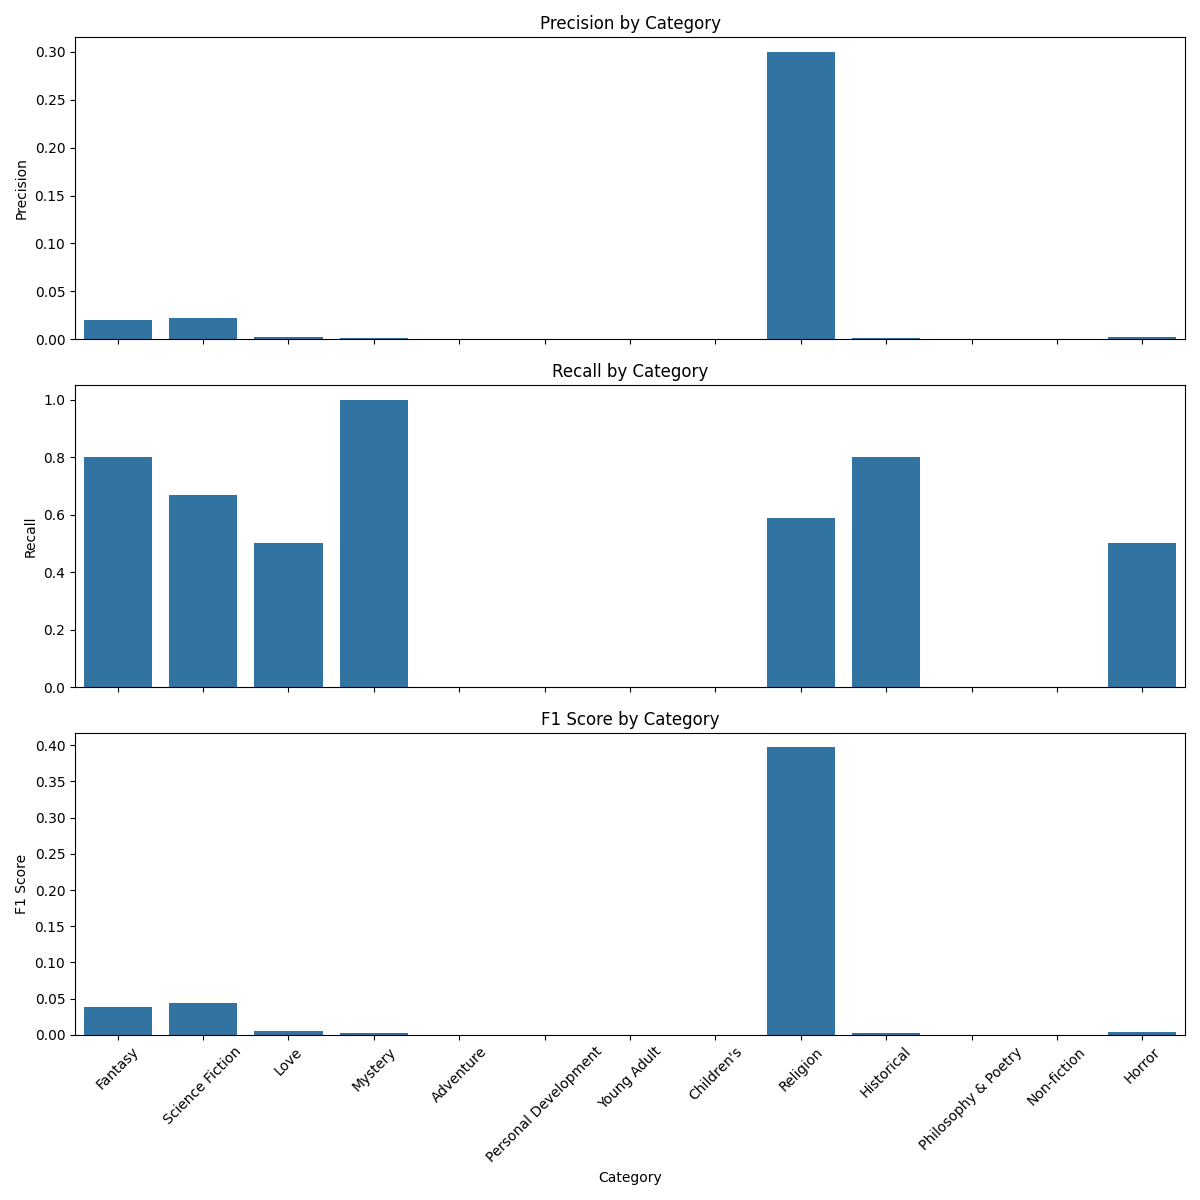
\includegraphics[scale=0.2]{refine_category_metrics_plot.png}
    
    \vspace{0.1cm}
    \tiny \textit{Results focus on high-confidence predictions rather than perfect recall across all categories}
  \end{column}
\end{columns}

\note{
  \begin{columns}[T]
    \begin{column}{0.49\textwidth}
      [TIMING: 1 minute - WHY TWO-TIER APPROACH:]
      \begin{itemize}
        \item "Zero-shot is powerful but not perfect"
        \item "Sometimes misses obvious genre indicators"
        \item "Fallback catches cases like book description containing 'wizard' but AI missed fantasy"
        \item "Hybrid approach gets best of both worlds"
      \end{itemize}
      
      \vspace{0.1cm}
      [EXPLAIN ZERO-SHOT (key concept):]
      \begin{itemize}
        \item "Zero-shot means no training examples needed"
        \item "Just ask BART: 'Is this book description about fantasy?'"
        \item "It understands the question and gives confidence score"
      \end{itemize}
      
      \vspace{0.1cm}
      [ADDRESS THE CHART HONESTLY:]
      \begin{itemize}
        \item "Yes, precision is low for some categories That's expected - I'm prioritizing high-confidence predictions"
        \item "Religious category shows best performance - clear vocabulary indicators"
        \item "This is proof-of-concept, not production system"
      \end{itemize}
    \end{column}
    
    \begin{column}{0.49\textwidth}
      [QUALITY CONTROL RATIONALE:]
      \begin{itemize}
        \item "200 chars minimum - need enough text for semantic analysis"
        \item "Confidence thresholds prevent low-quality predictions"
      \end{itemize}
      
      \vspace{0.1cm}
      [POTENTIAL QUESTIONS:]
      \begin{itemize}
        \item \textit{"Why BART-MNLI specifically?"} → "Pre-trained for natural language inference - exactly what we need for 'is this book about X?'"
        \item \textit{"How choose the 13 categories?"} → "Common book genres, could be expanded based on dataset"
        \item \textit{"What if zero-shot and fallback disagree?"} → "Take highest confidence, with preference for zero-shot"
        \item \textit{"Could you improve these metrics?"} → "Yes - larger training set, domain-specific fine-tuning, better thresholds"
      \end{itemize}
      
      \vspace{0.1cm}
      [TRANSITION:]
      \begin{itemize}
        \item "With categories assigned, the core challenge was semantic embedding..."
      \end{itemize}
    \end{column}
  \end{columns}
}

\end{frame}